% Created by tikzDevice version 0.10.1 on 2016-07-18 19:10:53
% !TEX encoding = UTF-8 Unicode
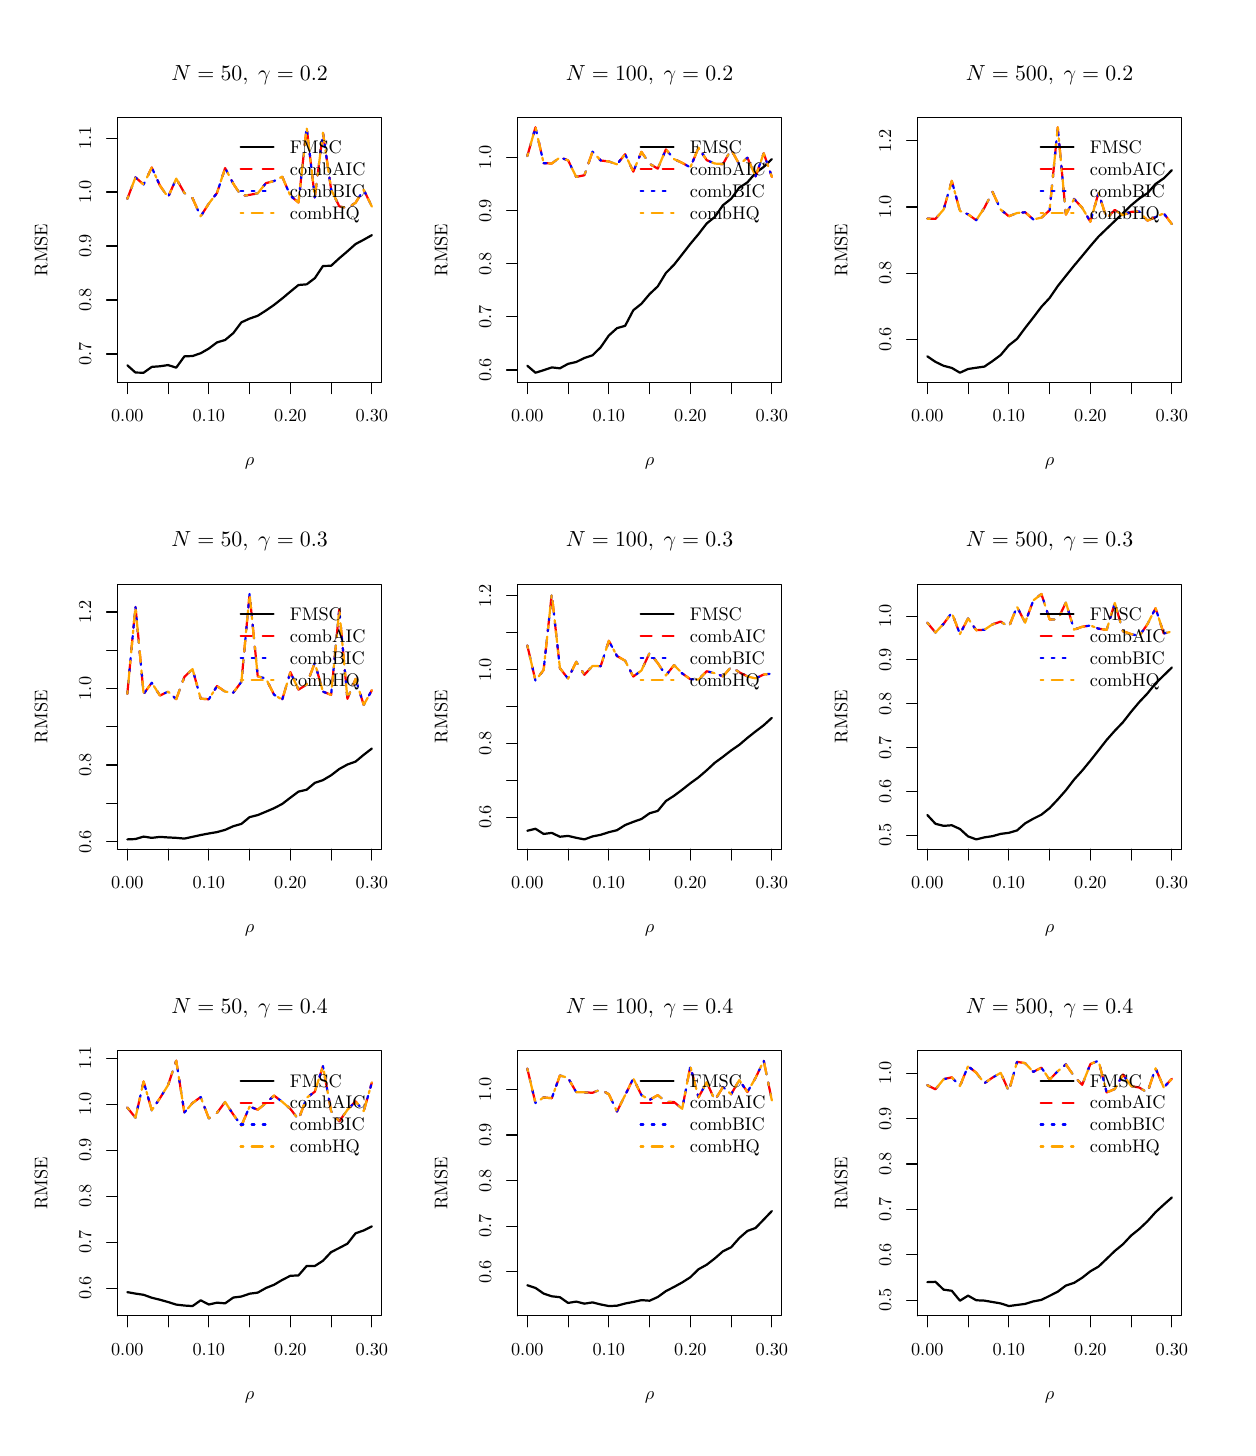
\begin{tikzpicture}[x=1pt,y=1pt]
\definecolor{fillColor}{RGB}{255,255,255}
\path[use as bounding box,fill=fillColor,fill opacity=0.00] (0,0) rectangle (433.62,505.89);
\begin{scope}
\path[clip] ( 32.47,377.65) rectangle (127.91,473.42);
\definecolor{drawColor}{RGB}{0,0,0}

\path[draw=drawColor,line width= 0.8pt,line join=round,line cap=round] ( 36.01,383.89) --
	( 38.95,381.26) --
	( 41.90,381.20) --
	( 44.84,383.31) --
	( 47.79,383.53) --
	( 50.73,383.97) --
	( 53.68,383.03) --
	( 56.63,387.11) --
	( 59.57,387.24) --
	( 62.52,388.24) --
	( 65.46,389.93) --
	( 68.41,392.16) --
	( 71.35,393.03) --
	( 74.30,395.51) --
	( 77.24,399.41) --
	( 80.19,400.76) --
	( 83.14,401.79) --
	( 86.08,403.66) --
	( 89.03,405.71) --
	( 91.97,408.02) --
	( 94.92,410.50) --
	( 97.86,412.90) --
	(100.81,413.14) --
	(103.75,415.36) --
	(106.70,419.77) --
	(109.65,419.85) --
	(112.59,422.55) --
	(115.54,425.07) --
	(118.48,427.70) --
	(121.43,429.26) --
	(124.37,430.91);
\end{scope}
\begin{scope}
\path[clip] (  0.00,  0.00) rectangle (433.62,505.89);
\definecolor{drawColor}{RGB}{0,0,0}

\path[draw=drawColor,line width= 0.4pt,line join=round,line cap=round] ( 36.01,377.65) -- (124.37,377.65);

\path[draw=drawColor,line width= 0.4pt,line join=round,line cap=round] ( 36.01,377.65) -- ( 36.01,373.69);

\path[draw=drawColor,line width= 0.4pt,line join=round,line cap=round] ( 50.73,377.65) -- ( 50.73,373.69);

\path[draw=drawColor,line width= 0.4pt,line join=round,line cap=round] ( 65.46,377.65) -- ( 65.46,373.69);

\path[draw=drawColor,line width= 0.4pt,line join=round,line cap=round] ( 80.19,377.65) -- ( 80.19,373.69);

\path[draw=drawColor,line width= 0.4pt,line join=round,line cap=round] ( 94.92,377.65) -- ( 94.92,373.69);

\path[draw=drawColor,line width= 0.4pt,line join=round,line cap=round] (109.65,377.65) -- (109.65,373.69);

\path[draw=drawColor,line width= 0.4pt,line join=round,line cap=round] (124.37,377.65) -- (124.37,373.69);

\node[text=drawColor,anchor=base,inner sep=0pt, outer sep=0pt, scale=  0.66] at ( 36.01,363.40) {0.00};

\node[text=drawColor,anchor=base,inner sep=0pt, outer sep=0pt, scale=  0.66] at ( 65.46,363.40) {0.10};

\node[text=drawColor,anchor=base,inner sep=0pt, outer sep=0pt, scale=  0.66] at ( 94.92,363.40) {0.20};

\node[text=drawColor,anchor=base,inner sep=0pt, outer sep=0pt, scale=  0.66] at (124.37,363.40) {0.30};

\path[draw=drawColor,line width= 0.4pt,line join=round,line cap=round] ( 32.47,387.98) -- ( 32.47,465.99);

\path[draw=drawColor,line width= 0.4pt,line join=round,line cap=round] ( 32.47,387.98) -- ( 28.51,387.98);

\path[draw=drawColor,line width= 0.4pt,line join=round,line cap=round] ( 32.47,407.48) -- ( 28.51,407.48);

\path[draw=drawColor,line width= 0.4pt,line join=round,line cap=round] ( 32.47,426.99) -- ( 28.51,426.99);

\path[draw=drawColor,line width= 0.4pt,line join=round,line cap=round] ( 32.47,446.49) -- ( 28.51,446.49);

\path[draw=drawColor,line width= 0.4pt,line join=round,line cap=round] ( 32.47,465.99) -- ( 28.51,465.99);

\node[text=drawColor,rotate= 90.00,anchor=base,inner sep=0pt, outer sep=0pt, scale=  0.66] at ( 22.97,387.98) {0.7};

\node[text=drawColor,rotate= 90.00,anchor=base,inner sep=0pt, outer sep=0pt, scale=  0.66] at ( 22.97,407.48) {0.8};

\node[text=drawColor,rotate= 90.00,anchor=base,inner sep=0pt, outer sep=0pt, scale=  0.66] at ( 22.97,426.99) {0.9};

\node[text=drawColor,rotate= 90.00,anchor=base,inner sep=0pt, outer sep=0pt, scale=  0.66] at ( 22.97,446.49) {1.0};

\node[text=drawColor,rotate= 90.00,anchor=base,inner sep=0pt, outer sep=0pt, scale=  0.66] at ( 22.97,465.99) {1.1};

\path[draw=drawColor,line width= 0.4pt,line join=round,line cap=round] ( 32.47,377.65) --
	(127.91,377.65) --
	(127.91,473.42) --
	( 32.47,473.42) --
	( 32.47,377.65);
\end{scope}
\begin{scope}
\path[clip] (  0.00,337.26) rectangle (144.54,505.89);
\definecolor{drawColor}{RGB}{0,0,0}

\node[text=drawColor,anchor=base,inner sep=0pt, outer sep=0pt, scale=  0.79] at ( 80.19,486.92) {\bfseries $N=50, \;\gamma=0.2$};

\node[text=drawColor,anchor=base,inner sep=0pt, outer sep=0pt, scale=  0.66] at ( 80.19,347.56) {$\rho$};

\node[text=drawColor,rotate= 90.00,anchor=base,inner sep=0pt, outer sep=0pt, scale=  0.66] at (  7.13,425.53) {RMSE};
\end{scope}
\begin{scope}
\path[clip] ( 32.47,377.65) rectangle (127.91,473.42);
\definecolor{drawColor}{RGB}{255,0,0}

\path[draw=drawColor,line width= 0.8pt,dash pattern=on 4pt off 4pt ,line join=round,line cap=round] ( 36.01,444.04) --
	( 38.95,451.78) --
	( 41.90,449.21) --
	( 44.84,455.37) --
	( 47.79,448.81) --
	( 50.73,444.63) --
	( 53.68,451.35) --
	( 56.63,446.14) --
	( 59.57,444.26) --
	( 62.52,437.71) --
	( 65.46,442.34) --
	( 68.41,446.14) --
	( 71.35,455.16) --
	( 74.30,449.51) --
	( 77.24,445.05) --
	( 80.19,445.47) --
	( 83.14,446.03) --
	( 86.08,449.70) --
	( 89.03,450.47) --
	( 91.97,452.05) --
	( 94.92,445.15) --
	( 97.86,442.71) --
	(100.81,469.87) --
	(103.75,444.54) --
	(106.70,467.95) --
	(109.65,447.43) --
	(112.59,441.33) --
	(115.54,440.61) --
	(118.48,442.63) --
	(121.43,447.34) --
	(124.37,441.23);
\definecolor{drawColor}{RGB}{0,0,255}

\path[draw=drawColor,line width= 0.8pt,dash pattern=on 1pt off 3pt ,line join=round,line cap=round] ( 36.01,444.04) --
	( 38.95,451.78) --
	( 41.90,449.21) --
	( 44.84,455.37) --
	( 47.79,448.81) --
	( 50.73,444.63) --
	( 53.68,451.35) --
	( 56.63,446.14) --
	( 59.57,444.26) --
	( 62.52,437.71) --
	( 65.46,442.34) --
	( 68.41,446.14) --
	( 71.35,455.16) --
	( 74.30,449.51) --
	( 77.24,445.05) --
	( 80.19,445.47) --
	( 83.14,446.03) --
	( 86.08,449.70) --
	( 89.03,450.47) --
	( 91.97,452.05) --
	( 94.92,445.15) --
	( 97.86,442.71) --
	(100.81,469.87) --
	(103.75,444.54) --
	(106.70,467.95) --
	(109.65,447.43) --
	(112.59,441.33) --
	(115.54,440.61) --
	(118.48,442.63) --
	(121.43,447.34) --
	(124.37,441.23);
\definecolor{drawColor}{RGB}{255,165,0}

\path[draw=drawColor,line width= 0.8pt,dash pattern=on 1pt off 3pt on 4pt off 3pt ,line join=round,line cap=round] ( 36.01,444.04) --
	( 38.95,451.78) --
	( 41.90,449.21) --
	( 44.84,455.37) --
	( 47.79,448.81) --
	( 50.73,444.63) --
	( 53.68,451.35) --
	( 56.63,446.14) --
	( 59.57,444.26) --
	( 62.52,437.71) --
	( 65.46,442.34) --
	( 68.41,446.14) --
	( 71.35,455.16) --
	( 74.30,449.51) --
	( 77.24,445.05) --
	( 80.19,445.47) --
	( 83.14,446.03) --
	( 86.08,449.70) --
	( 89.03,450.47) --
	( 91.97,452.05) --
	( 94.92,445.15) --
	( 97.86,442.71) --
	(100.81,469.87) --
	(103.75,444.54) --
	(106.70,467.95) --
	(109.65,447.43) --
	(112.59,441.33) --
	(115.54,440.61) --
	(118.48,442.63) --
	(121.43,447.34) --
	(124.37,441.23);
\definecolor{drawColor}{RGB}{0,0,0}

\path[draw=drawColor,line width= 0.8pt,line join=round,line cap=round] ( 76.94,462.63) -- ( 88.82,462.63);
\definecolor{drawColor}{RGB}{255,0,0}

\path[draw=drawColor,line width= 0.8pt,dash pattern=on 4pt off 4pt ,line join=round,line cap=round] ( 76.94,454.71) -- ( 88.82,454.71);
\definecolor{drawColor}{RGB}{0,0,255}

\path[draw=drawColor,line width= 0.8pt,dash pattern=on 1pt off 3pt ,line join=round,line cap=round] ( 76.94,446.79) -- ( 88.82,446.79);
\definecolor{drawColor}{RGB}{255,165,0}

\path[draw=drawColor,line width= 0.8pt,dash pattern=on 1pt off 3pt on 4pt off 3pt ,line join=round,line cap=round] ( 76.94,438.87) -- ( 88.82,438.87);
\definecolor{drawColor}{RGB}{0,0,0}

\node[text=drawColor,anchor=base west,inner sep=0pt, outer sep=0pt, scale=  0.66] at ( 94.76,460.35) {FMSC};

\node[text=drawColor,anchor=base west,inner sep=0pt, outer sep=0pt, scale=  0.66] at ( 94.76,452.43) {combAIC};

\node[text=drawColor,anchor=base west,inner sep=0pt, outer sep=0pt, scale=  0.66] at ( 94.76,444.51) {combBIC};

\node[text=drawColor,anchor=base west,inner sep=0pt, outer sep=0pt, scale=  0.66] at ( 94.76,436.59) {combHQ};
\end{scope}
\begin{scope}
\path[clip] (177.01,377.65) rectangle (272.45,473.42);
\definecolor{drawColor}{RGB}{0,0,0}

\path[draw=drawColor,line width= 0.8pt,line join=round,line cap=round] (180.55,383.73) --
	(183.49,381.20) --
	(186.44,382.11) --
	(189.38,383.12) --
	(192.33,382.80) --
	(195.27,384.41) --
	(198.22,385.08) --
	(201.17,386.53) --
	(204.11,387.49) --
	(207.06,390.40) --
	(210.00,394.65) --
	(212.95,397.31) --
	(215.89,398.15) --
	(218.84,403.78) --
	(221.78,406.12) --
	(224.73,409.62) --
	(227.68,412.40) --
	(230.62,417.23) --
	(233.57,420.24) --
	(236.51,423.97) --
	(239.46,427.77) --
	(242.40,431.28) --
	(245.35,435.12) --
	(248.29,437.48) --
	(251.24,441.74) --
	(254.19,444.05) --
	(257.13,448.06) --
	(260.08,449.99) --
	(263.02,453.40) --
	(265.97,455.56) --
	(268.91,458.41);
\end{scope}
\begin{scope}
\path[clip] (  0.00,  0.00) rectangle (433.62,505.89);
\definecolor{drawColor}{RGB}{0,0,0}

\path[draw=drawColor,line width= 0.4pt,line join=round,line cap=round] (180.55,377.65) -- (268.91,377.65);

\path[draw=drawColor,line width= 0.4pt,line join=round,line cap=round] (180.55,377.65) -- (180.55,373.69);

\path[draw=drawColor,line width= 0.4pt,line join=round,line cap=round] (195.27,377.65) -- (195.27,373.69);

\path[draw=drawColor,line width= 0.4pt,line join=round,line cap=round] (210.00,377.65) -- (210.00,373.69);

\path[draw=drawColor,line width= 0.4pt,line join=round,line cap=round] (224.73,377.65) -- (224.73,373.69);

\path[draw=drawColor,line width= 0.4pt,line join=round,line cap=round] (239.46,377.65) -- (239.46,373.69);

\path[draw=drawColor,line width= 0.4pt,line join=round,line cap=round] (254.19,377.65) -- (254.19,373.69);

\path[draw=drawColor,line width= 0.4pt,line join=round,line cap=round] (268.91,377.65) -- (268.91,373.69);

\node[text=drawColor,anchor=base,inner sep=0pt, outer sep=0pt, scale=  0.66] at (180.55,363.40) {0.00};

\node[text=drawColor,anchor=base,inner sep=0pt, outer sep=0pt, scale=  0.66] at (210.00,363.40) {0.10};

\node[text=drawColor,anchor=base,inner sep=0pt, outer sep=0pt, scale=  0.66] at (239.46,363.40) {0.20};

\node[text=drawColor,anchor=base,inner sep=0pt, outer sep=0pt, scale=  0.66] at (268.91,363.40) {0.30};

\path[draw=drawColor,line width= 0.4pt,line join=round,line cap=round] (177.01,382.19) -- (177.01,459.01);

\path[draw=drawColor,line width= 0.4pt,line join=round,line cap=round] (177.01,382.19) -- (173.05,382.19);

\path[draw=drawColor,line width= 0.4pt,line join=round,line cap=round] (177.01,401.40) -- (173.05,401.40);

\path[draw=drawColor,line width= 0.4pt,line join=round,line cap=round] (177.01,420.60) -- (173.05,420.60);

\path[draw=drawColor,line width= 0.4pt,line join=round,line cap=round] (177.01,439.81) -- (173.05,439.81);

\path[draw=drawColor,line width= 0.4pt,line join=round,line cap=round] (177.01,459.01) -- (173.05,459.01);

\node[text=drawColor,rotate= 90.00,anchor=base,inner sep=0pt, outer sep=0pt, scale=  0.66] at (167.51,382.19) {0.6};

\node[text=drawColor,rotate= 90.00,anchor=base,inner sep=0pt, outer sep=0pt, scale=  0.66] at (167.51,401.40) {0.7};

\node[text=drawColor,rotate= 90.00,anchor=base,inner sep=0pt, outer sep=0pt, scale=  0.66] at (167.51,420.60) {0.8};

\node[text=drawColor,rotate= 90.00,anchor=base,inner sep=0pt, outer sep=0pt, scale=  0.66] at (167.51,439.81) {0.9};

\node[text=drawColor,rotate= 90.00,anchor=base,inner sep=0pt, outer sep=0pt, scale=  0.66] at (167.51,459.01) {1.0};

\path[draw=drawColor,line width= 0.4pt,line join=round,line cap=round] (177.01,377.65) --
	(272.45,377.65) --
	(272.45,473.42) --
	(177.01,473.42) --
	(177.01,377.65);
\end{scope}
\begin{scope}
\path[clip] (144.54,337.26) rectangle (289.08,505.89);
\definecolor{drawColor}{RGB}{0,0,0}

\node[text=drawColor,anchor=base,inner sep=0pt, outer sep=0pt, scale=  0.79] at (224.73,486.92) {\bfseries $N=100, \;\gamma=0.2$};

\node[text=drawColor,anchor=base,inner sep=0pt, outer sep=0pt, scale=  0.66] at (224.73,347.56) {$\rho$};

\node[text=drawColor,rotate= 90.00,anchor=base,inner sep=0pt, outer sep=0pt, scale=  0.66] at (151.67,425.53) {RMSE};
\end{scope}
\begin{scope}
\path[clip] (177.01,377.65) rectangle (272.45,473.42);
\definecolor{drawColor}{RGB}{255,0,0}

\path[draw=drawColor,line width= 0.8pt,dash pattern=on 4pt off 4pt ,line join=round,line cap=round] (180.55,459.51) --
	(183.49,469.87) --
	(186.44,456.92) --
	(189.38,456.80) --
	(192.33,459.00) --
	(195.27,457.95) --
	(198.22,451.96) --
	(201.17,452.56) --
	(204.11,461.09) --
	(207.06,457.89) --
	(210.00,457.53) --
	(212.95,456.52) --
	(215.89,460.16) --
	(218.84,453.86) --
	(221.78,461.01) --
	(224.73,456.69) --
	(227.68,454.93) --
	(230.62,461.89) --
	(233.57,458.40) --
	(236.51,457.04) --
	(239.46,455.38) --
	(242.40,462.52) --
	(245.35,458.02) --
	(248.29,456.79) --
	(251.24,456.60) --
	(254.19,461.86) --
	(257.13,456.50) --
	(260.08,458.87) --
	(263.02,452.15) --
	(265.97,460.49) --
	(268.91,451.99);
\definecolor{drawColor}{RGB}{0,0,255}

\path[draw=drawColor,line width= 0.8pt,dash pattern=on 1pt off 3pt ,line join=round,line cap=round] (180.55,459.51) --
	(183.49,469.87) --
	(186.44,456.92) --
	(189.38,456.80) --
	(192.33,459.00) --
	(195.27,457.95) --
	(198.22,451.96) --
	(201.17,452.56) --
	(204.11,461.09) --
	(207.06,457.89) --
	(210.00,457.53) --
	(212.95,456.52) --
	(215.89,460.16) --
	(218.84,453.86) --
	(221.78,461.01) --
	(224.73,456.69) --
	(227.68,454.93) --
	(230.62,461.89) --
	(233.57,458.40) --
	(236.51,457.04) --
	(239.46,455.38) --
	(242.40,462.52) --
	(245.35,458.02) --
	(248.29,456.79) --
	(251.24,456.60) --
	(254.19,461.86) --
	(257.13,456.50) --
	(260.08,458.87) --
	(263.02,452.15) --
	(265.97,460.49) --
	(268.91,451.99);
\definecolor{drawColor}{RGB}{255,165,0}

\path[draw=drawColor,line width= 0.8pt,dash pattern=on 1pt off 3pt on 4pt off 3pt ,line join=round,line cap=round] (180.55,459.51) --
	(183.49,469.87) --
	(186.44,456.92) --
	(189.38,456.80) --
	(192.33,459.00) --
	(195.27,457.95) --
	(198.22,451.96) --
	(201.17,452.56) --
	(204.11,461.09) --
	(207.06,457.89) --
	(210.00,457.53) --
	(212.95,456.52) --
	(215.89,460.16) --
	(218.84,453.86) --
	(221.78,461.01) --
	(224.73,456.69) --
	(227.68,454.93) --
	(230.62,461.89) --
	(233.57,458.40) --
	(236.51,457.04) --
	(239.46,455.38) --
	(242.40,462.52) --
	(245.35,458.02) --
	(248.29,456.79) --
	(251.24,456.60) --
	(254.19,461.86) --
	(257.13,456.50) --
	(260.08,458.87) --
	(263.02,452.15) --
	(265.97,460.49) --
	(268.91,451.99);
\definecolor{drawColor}{RGB}{0,0,0}

\path[draw=drawColor,line width= 0.8pt,line join=round,line cap=round] (221.48,462.63) -- (233.36,462.63);
\definecolor{drawColor}{RGB}{255,0,0}

\path[draw=drawColor,line width= 0.8pt,dash pattern=on 4pt off 4pt ,line join=round,line cap=round] (221.48,454.71) -- (233.36,454.71);
\definecolor{drawColor}{RGB}{0,0,255}

\path[draw=drawColor,line width= 0.8pt,dash pattern=on 1pt off 3pt ,line join=round,line cap=round] (221.48,446.79) -- (233.36,446.79);
\definecolor{drawColor}{RGB}{255,165,0}

\path[draw=drawColor,line width= 0.8pt,dash pattern=on 1pt off 3pt on 4pt off 3pt ,line join=round,line cap=round] (221.48,438.87) -- (233.36,438.87);
\definecolor{drawColor}{RGB}{0,0,0}

\node[text=drawColor,anchor=base west,inner sep=0pt, outer sep=0pt, scale=  0.66] at (239.30,460.35) {FMSC};

\node[text=drawColor,anchor=base west,inner sep=0pt, outer sep=0pt, scale=  0.66] at (239.30,452.43) {combAIC};

\node[text=drawColor,anchor=base west,inner sep=0pt, outer sep=0pt, scale=  0.66] at (239.30,444.51) {combBIC};

\node[text=drawColor,anchor=base west,inner sep=0pt, outer sep=0pt, scale=  0.66] at (239.30,436.59) {combHQ};
\end{scope}
\begin{scope}
\path[clip] (321.55,377.65) rectangle (416.99,473.42);
\definecolor{drawColor}{RGB}{0,0,0}

\path[draw=drawColor,line width= 0.8pt,line join=round,line cap=round] (325.09,387.12) --
	(328.03,385.12) --
	(330.98,383.70) --
	(333.92,382.94) --
	(336.87,381.20) --
	(339.81,382.55) --
	(342.76,383.00) --
	(345.71,383.42) --
	(348.65,385.41) --
	(351.60,387.60) --
	(354.54,391.09) --
	(357.49,393.41) --
	(360.43,397.36) --
	(363.38,401.15) --
	(366.32,405.03) --
	(369.27,408.20) --
	(372.22,412.50) --
	(375.16,416.22) --
	(378.11,419.88) --
	(381.05,423.39) --
	(384.00,426.96) --
	(386.94,430.38) --
	(389.89,433.23) --
	(392.83,436.04) --
	(395.78,438.81) --
	(398.73,441.70) --
	(401.67,444.15) --
	(404.62,446.06) --
	(407.56,449.42) --
	(410.51,451.43) --
	(413.45,454.39);
\end{scope}
\begin{scope}
\path[clip] (  0.00,  0.00) rectangle (433.62,505.89);
\definecolor{drawColor}{RGB}{0,0,0}

\path[draw=drawColor,line width= 0.4pt,line join=round,line cap=round] (325.09,377.65) -- (413.45,377.65);

\path[draw=drawColor,line width= 0.4pt,line join=round,line cap=round] (325.09,377.65) -- (325.09,373.69);

\path[draw=drawColor,line width= 0.4pt,line join=round,line cap=round] (339.81,377.65) -- (339.81,373.69);

\path[draw=drawColor,line width= 0.4pt,line join=round,line cap=round] (354.54,377.65) -- (354.54,373.69);

\path[draw=drawColor,line width= 0.4pt,line join=round,line cap=round] (369.27,377.65) -- (369.27,373.69);

\path[draw=drawColor,line width= 0.4pt,line join=round,line cap=round] (384.00,377.65) -- (384.00,373.69);

\path[draw=drawColor,line width= 0.4pt,line join=round,line cap=round] (398.73,377.65) -- (398.73,373.69);

\path[draw=drawColor,line width= 0.4pt,line join=round,line cap=round] (413.45,377.65) -- (413.45,373.69);

\node[text=drawColor,anchor=base,inner sep=0pt, outer sep=0pt, scale=  0.66] at (325.09,363.40) {0.00};

\node[text=drawColor,anchor=base,inner sep=0pt, outer sep=0pt, scale=  0.66] at (354.54,363.40) {0.10};

\node[text=drawColor,anchor=base,inner sep=0pt, outer sep=0pt, scale=  0.66] at (384.00,363.40) {0.20};

\node[text=drawColor,anchor=base,inner sep=0pt, outer sep=0pt, scale=  0.66] at (413.45,363.40) {0.30};

\path[draw=drawColor,line width= 0.4pt,line join=round,line cap=round] (321.55,393.24) -- (321.55,465.04);

\path[draw=drawColor,line width= 0.4pt,line join=round,line cap=round] (321.55,393.24) -- (317.59,393.24);

\path[draw=drawColor,line width= 0.4pt,line join=round,line cap=round] (321.55,417.17) -- (317.59,417.17);

\path[draw=drawColor,line width= 0.4pt,line join=round,line cap=round] (321.55,441.10) -- (317.59,441.10);

\path[draw=drawColor,line width= 0.4pt,line join=round,line cap=round] (321.55,465.04) -- (317.59,465.04);

\node[text=drawColor,rotate= 90.00,anchor=base,inner sep=0pt, outer sep=0pt, scale=  0.66] at (312.05,393.24) {0.6};

\node[text=drawColor,rotate= 90.00,anchor=base,inner sep=0pt, outer sep=0pt, scale=  0.66] at (312.05,417.17) {0.8};

\node[text=drawColor,rotate= 90.00,anchor=base,inner sep=0pt, outer sep=0pt, scale=  0.66] at (312.05,441.10) {1.0};

\node[text=drawColor,rotate= 90.00,anchor=base,inner sep=0pt, outer sep=0pt, scale=  0.66] at (312.05,465.04) {1.2};

\path[draw=drawColor,line width= 0.4pt,line join=round,line cap=round] (321.55,377.65) --
	(416.99,377.65) --
	(416.99,473.42) --
	(321.55,473.42) --
	(321.55,377.65);
\end{scope}
\begin{scope}
\path[clip] (289.08,337.26) rectangle (433.62,505.89);
\definecolor{drawColor}{RGB}{0,0,0}

\node[text=drawColor,anchor=base,inner sep=0pt, outer sep=0pt, scale=  0.79] at (369.27,486.92) {\bfseries $N=500, \;\gamma=0.2$};

\node[text=drawColor,anchor=base,inner sep=0pt, outer sep=0pt, scale=  0.66] at (369.27,347.56) {$\rho$};

\node[text=drawColor,rotate= 90.00,anchor=base,inner sep=0pt, outer sep=0pt, scale=  0.66] at (296.21,425.53) {RMSE};
\end{scope}
\begin{scope}
\path[clip] (321.55,377.65) rectangle (416.99,473.42);
\definecolor{drawColor}{RGB}{255,0,0}

\path[draw=drawColor,line width= 0.8pt,dash pattern=on 4pt off 4pt ,line join=round,line cap=round] (325.09,436.85) --
	(328.03,436.79) --
	(330.98,440.18) --
	(333.92,450.54) --
	(336.87,439.66) --
	(339.81,438.43) --
	(342.76,436.32) --
	(345.71,440.81) --
	(348.65,446.52) --
	(351.60,440.15) --
	(354.54,437.74) --
	(357.49,438.91) --
	(360.43,439.18) --
	(363.38,436.60) --
	(366.32,437.24) --
	(369.27,439.90) --
	(372.22,469.87) --
	(375.16,438.33) --
	(378.11,443.99) --
	(381.05,440.80) --
	(384.00,435.77) --
	(386.94,446.17) --
	(389.89,436.95) --
	(392.83,440.02) --
	(395.78,438.11) --
	(398.73,439.32) --
	(401.67,439.48) --
	(404.62,436.16) --
	(407.56,437.44) --
	(410.51,438.80) --
	(413.45,434.91);
\definecolor{drawColor}{RGB}{0,0,255}

\path[draw=drawColor,line width= 0.8pt,dash pattern=on 1pt off 3pt ,line join=round,line cap=round] (325.09,436.85) --
	(328.03,436.79) --
	(330.98,440.18) --
	(333.92,450.54) --
	(336.87,439.66) --
	(339.81,438.43) --
	(342.76,436.32) --
	(345.71,440.81) --
	(348.65,446.52) --
	(351.60,440.15) --
	(354.54,437.74) --
	(357.49,438.91) --
	(360.43,439.18) --
	(363.38,436.60) --
	(366.32,437.24) --
	(369.27,439.90) --
	(372.22,469.87) --
	(375.16,438.33) --
	(378.11,443.99) --
	(381.05,440.80) --
	(384.00,435.77) --
	(386.94,446.17) --
	(389.89,436.95) --
	(392.83,440.02) --
	(395.78,438.11) --
	(398.73,439.32) --
	(401.67,439.48) --
	(404.62,436.16) --
	(407.56,437.44) --
	(410.51,438.80) --
	(413.45,434.91);
\definecolor{drawColor}{RGB}{255,165,0}

\path[draw=drawColor,line width= 0.8pt,dash pattern=on 1pt off 3pt on 4pt off 3pt ,line join=round,line cap=round] (325.09,436.85) --
	(328.03,436.79) --
	(330.98,440.18) --
	(333.92,450.54) --
	(336.87,439.66) --
	(339.81,438.43) --
	(342.76,436.32) --
	(345.71,440.81) --
	(348.65,446.52) --
	(351.60,440.15) --
	(354.54,437.74) --
	(357.49,438.91) --
	(360.43,439.18) --
	(363.38,436.60) --
	(366.32,437.24) --
	(369.27,439.90) --
	(372.22,469.87) --
	(375.16,438.33) --
	(378.11,443.99) --
	(381.05,440.80) --
	(384.00,435.77) --
	(386.94,446.17) --
	(389.89,436.95) --
	(392.83,440.02) --
	(395.78,438.11) --
	(398.73,439.32) --
	(401.67,439.48) --
	(404.62,436.16) --
	(407.56,437.44) --
	(410.51,438.80) --
	(413.45,434.91);
\definecolor{drawColor}{RGB}{0,0,0}

\path[draw=drawColor,line width= 0.8pt,line join=round,line cap=round] (366.02,462.63) -- (377.90,462.63);
\definecolor{drawColor}{RGB}{255,0,0}

\path[draw=drawColor,line width= 0.8pt,dash pattern=on 4pt off 4pt ,line join=round,line cap=round] (366.02,454.71) -- (377.90,454.71);
\definecolor{drawColor}{RGB}{0,0,255}

\path[draw=drawColor,line width= 0.8pt,dash pattern=on 1pt off 3pt ,line join=round,line cap=round] (366.02,446.79) -- (377.90,446.79);
\definecolor{drawColor}{RGB}{255,165,0}

\path[draw=drawColor,line width= 0.8pt,dash pattern=on 1pt off 3pt on 4pt off 3pt ,line join=round,line cap=round] (366.02,438.87) -- (377.90,438.87);
\definecolor{drawColor}{RGB}{0,0,0}

\node[text=drawColor,anchor=base west,inner sep=0pt, outer sep=0pt, scale=  0.66] at (383.84,460.35) {FMSC};

\node[text=drawColor,anchor=base west,inner sep=0pt, outer sep=0pt, scale=  0.66] at (383.84,452.43) {combAIC};

\node[text=drawColor,anchor=base west,inner sep=0pt, outer sep=0pt, scale=  0.66] at (383.84,444.51) {combBIC};

\node[text=drawColor,anchor=base west,inner sep=0pt, outer sep=0pt, scale=  0.66] at (383.84,436.59) {combHQ};
\end{scope}
\begin{scope}
\path[clip] ( 32.47,209.02) rectangle (127.91,304.79);
\definecolor{drawColor}{RGB}{0,0,0}

\path[draw=drawColor,line width= 0.8pt,line join=round,line cap=round] ( 36.01,212.57) --
	( 38.95,212.70) --
	( 41.90,213.59) --
	( 44.84,213.12) --
	( 47.79,213.48) --
	( 50.73,213.28) --
	( 53.68,213.13) --
	( 56.63,212.86) --
	( 59.57,213.50) --
	( 62.52,214.15) --
	( 65.46,214.71) --
	( 68.41,215.21) --
	( 71.35,216.01) --
	( 74.30,217.33) --
	( 77.24,218.17) --
	( 80.19,220.62) --
	( 83.14,221.36) --
	( 86.08,222.58) --
	( 89.03,223.84) --
	( 91.97,225.38) --
	( 94.92,227.64) --
	( 97.86,229.84) --
	(100.81,230.52) --
	(103.75,232.99) --
	(106.70,233.99) --
	(109.65,235.74) --
	(112.59,238.00) --
	(115.54,239.63) --
	(118.48,240.68) --
	(121.43,243.13) --
	(124.37,245.41);
\end{scope}
\begin{scope}
\path[clip] (  0.00,  0.00) rectangle (433.62,505.89);
\definecolor{drawColor}{RGB}{0,0,0}

\path[draw=drawColor,line width= 0.4pt,line join=round,line cap=round] ( 36.01,209.02) -- (124.37,209.02);

\path[draw=drawColor,line width= 0.4pt,line join=round,line cap=round] ( 36.01,209.02) -- ( 36.01,205.06);

\path[draw=drawColor,line width= 0.4pt,line join=round,line cap=round] ( 50.73,209.02) -- ( 50.73,205.06);

\path[draw=drawColor,line width= 0.4pt,line join=round,line cap=round] ( 65.46,209.02) -- ( 65.46,205.06);

\path[draw=drawColor,line width= 0.4pt,line join=round,line cap=round] ( 80.19,209.02) -- ( 80.19,205.06);

\path[draw=drawColor,line width= 0.4pt,line join=round,line cap=round] ( 94.92,209.02) -- ( 94.92,205.06);

\path[draw=drawColor,line width= 0.4pt,line join=round,line cap=round] (109.65,209.02) -- (109.65,205.06);

\path[draw=drawColor,line width= 0.4pt,line join=round,line cap=round] (124.37,209.02) -- (124.37,205.06);

\node[text=drawColor,anchor=base,inner sep=0pt, outer sep=0pt, scale=  0.66] at ( 36.01,194.77) {0.00};

\node[text=drawColor,anchor=base,inner sep=0pt, outer sep=0pt, scale=  0.66] at ( 65.46,194.77) {0.10};

\node[text=drawColor,anchor=base,inner sep=0pt, outer sep=0pt, scale=  0.66] at ( 94.92,194.77) {0.20};

\node[text=drawColor,anchor=base,inner sep=0pt, outer sep=0pt, scale=  0.66] at (124.37,194.77) {0.30};

\path[draw=drawColor,line width= 0.4pt,line join=round,line cap=round] ( 32.47,211.79) -- ( 32.47,294.75);

\path[draw=drawColor,line width= 0.4pt,line join=round,line cap=round] ( 32.47,211.79) -- ( 28.51,211.79);

\path[draw=drawColor,line width= 0.4pt,line join=round,line cap=round] ( 32.47,225.62) -- ( 28.51,225.62);

\path[draw=drawColor,line width= 0.4pt,line join=round,line cap=round] ( 32.47,239.44) -- ( 28.51,239.44);

\path[draw=drawColor,line width= 0.4pt,line join=round,line cap=round] ( 32.47,253.27) -- ( 28.51,253.27);

\path[draw=drawColor,line width= 0.4pt,line join=round,line cap=round] ( 32.47,267.09) -- ( 28.51,267.09);

\path[draw=drawColor,line width= 0.4pt,line join=round,line cap=round] ( 32.47,280.92) -- ( 28.51,280.92);

\path[draw=drawColor,line width= 0.4pt,line join=round,line cap=round] ( 32.47,294.75) -- ( 28.51,294.75);

\node[text=drawColor,rotate= 90.00,anchor=base,inner sep=0pt, outer sep=0pt, scale=  0.66] at ( 22.97,211.79) {0.6};

\node[text=drawColor,rotate= 90.00,anchor=base,inner sep=0pt, outer sep=0pt, scale=  0.66] at ( 22.97,239.44) {0.8};

\node[text=drawColor,rotate= 90.00,anchor=base,inner sep=0pt, outer sep=0pt, scale=  0.66] at ( 22.97,267.09) {1.0};

\node[text=drawColor,rotate= 90.00,anchor=base,inner sep=0pt, outer sep=0pt, scale=  0.66] at ( 22.97,294.75) {1.2};

\path[draw=drawColor,line width= 0.4pt,line join=round,line cap=round] ( 32.47,209.02) --
	(127.91,209.02) --
	(127.91,304.79) --
	( 32.47,304.79) --
	( 32.47,209.02);
\end{scope}
\begin{scope}
\path[clip] (  0.00,168.63) rectangle (144.54,337.26);
\definecolor{drawColor}{RGB}{0,0,0}

\node[text=drawColor,anchor=base,inner sep=0pt, outer sep=0pt, scale=  0.79] at ( 80.19,318.29) {\bfseries $N=50, \;\gamma=0.3$};

\node[text=drawColor,anchor=base,inner sep=0pt, outer sep=0pt, scale=  0.66] at ( 80.19,178.93) {$\rho$};

\node[text=drawColor,rotate= 90.00,anchor=base,inner sep=0pt, outer sep=0pt, scale=  0.66] at (  7.13,256.90) {RMSE};
\end{scope}
\begin{scope}
\path[clip] ( 32.47,209.02) rectangle (127.91,304.79);
\definecolor{drawColor}{RGB}{255,0,0}

\path[draw=drawColor,line width= 0.8pt,dash pattern=on 4pt off 4pt ,line join=round,line cap=round] ( 36.01,265.18) --
	( 38.95,296.79) --
	( 41.90,265.13) --
	( 44.84,269.18) --
	( 47.79,264.55) --
	( 50.73,265.97) --
	( 53.68,263.25) --
	( 56.63,271.29) --
	( 59.57,274.12) --
	( 62.52,263.42) --
	( 65.46,263.21) --
	( 68.41,267.96) --
	( 71.35,265.97) --
	( 74.30,265.59) --
	( 77.24,269.52) --
	( 80.19,301.24) --
	( 83.14,271.47) --
	( 86.08,270.72) --
	( 89.03,264.84) --
	( 91.97,263.05) --
	( 94.92,273.00) --
	( 97.86,266.68) --
	(100.81,268.52) --
	(103.75,276.37) --
	(106.70,265.97) --
	(109.65,264.79) --
	(112.59,295.63) --
	(115.54,263.37) --
	(118.48,270.56) --
	(121.43,261.16) --
	(124.37,266.47);
\definecolor{drawColor}{RGB}{0,0,255}

\path[draw=drawColor,line width= 0.8pt,dash pattern=on 1pt off 3pt ,line join=round,line cap=round] ( 36.01,265.18) --
	( 38.95,296.79) --
	( 41.90,265.13) --
	( 44.84,269.18) --
	( 47.79,264.55) --
	( 50.73,265.97) --
	( 53.68,263.25) --
	( 56.63,271.29) --
	( 59.57,274.12) --
	( 62.52,263.42) --
	( 65.46,263.21) --
	( 68.41,267.96) --
	( 71.35,265.97) --
	( 74.30,265.59) --
	( 77.24,269.52) --
	( 80.19,301.24) --
	( 83.14,271.47) --
	( 86.08,270.72) --
	( 89.03,264.84) --
	( 91.97,263.05) --
	( 94.92,273.00) --
	( 97.86,266.68) --
	(100.81,268.52) --
	(103.75,276.37) --
	(106.70,265.97) --
	(109.65,264.79) --
	(112.59,295.63) --
	(115.54,263.37) --
	(118.48,270.56) --
	(121.43,261.16) --
	(124.37,266.47);
\definecolor{drawColor}{RGB}{255,165,0}

\path[draw=drawColor,line width= 0.8pt,dash pattern=on 1pt off 3pt on 4pt off 3pt ,line join=round,line cap=round] ( 36.01,265.18) --
	( 38.95,296.79) --
	( 41.90,265.13) --
	( 44.84,269.18) --
	( 47.79,264.55) --
	( 50.73,265.97) --
	( 53.68,263.25) --
	( 56.63,271.29) --
	( 59.57,274.12) --
	( 62.52,263.42) --
	( 65.46,263.21) --
	( 68.41,267.96) --
	( 71.35,265.97) --
	( 74.30,265.59) --
	( 77.24,269.52) --
	( 80.19,301.24) --
	( 83.14,271.47) --
	( 86.08,270.72) --
	( 89.03,264.84) --
	( 91.97,263.05) --
	( 94.92,273.00) --
	( 97.86,266.68) --
	(100.81,268.52) --
	(103.75,276.37) --
	(106.70,265.97) --
	(109.65,264.79) --
	(112.59,295.63) --
	(115.54,263.37) --
	(118.48,270.56) --
	(121.43,261.16) --
	(124.37,266.47);
\definecolor{drawColor}{RGB}{0,0,0}

\path[draw=drawColor,line width= 0.8pt,line join=round,line cap=round] ( 76.94,294.00) -- ( 88.82,294.00);
\definecolor{drawColor}{RGB}{255,0,0}

\path[draw=drawColor,line width= 0.8pt,dash pattern=on 4pt off 4pt ,line join=round,line cap=round] ( 76.94,286.08) -- ( 88.82,286.08);
\definecolor{drawColor}{RGB}{0,0,255}

\path[draw=drawColor,line width= 0.8pt,dash pattern=on 1pt off 3pt ,line join=round,line cap=round] ( 76.94,278.16) -- ( 88.82,278.16);
\definecolor{drawColor}{RGB}{255,165,0}

\path[draw=drawColor,line width= 0.8pt,dash pattern=on 1pt off 3pt on 4pt off 3pt ,line join=round,line cap=round] ( 76.94,270.24) -- ( 88.82,270.24);
\definecolor{drawColor}{RGB}{0,0,0}

\node[text=drawColor,anchor=base west,inner sep=0pt, outer sep=0pt, scale=  0.66] at ( 94.76,291.72) {FMSC};

\node[text=drawColor,anchor=base west,inner sep=0pt, outer sep=0pt, scale=  0.66] at ( 94.76,283.80) {combAIC};

\node[text=drawColor,anchor=base west,inner sep=0pt, outer sep=0pt, scale=  0.66] at ( 94.76,275.88) {combBIC};

\node[text=drawColor,anchor=base west,inner sep=0pt, outer sep=0pt, scale=  0.66] at ( 94.76,267.96) {combHQ};
\end{scope}
\begin{scope}
\path[clip] (177.01,209.02) rectangle (272.45,304.79);
\definecolor{drawColor}{RGB}{0,0,0}

\path[draw=drawColor,line width= 0.8pt,line join=round,line cap=round] (180.55,215.69) --
	(183.49,216.41) --
	(186.44,214.54) --
	(189.38,214.92) --
	(192.33,213.53) --
	(195.27,213.84) --
	(198.22,213.15) --
	(201.17,212.57) --
	(204.11,213.65) --
	(207.06,214.23) --
	(210.00,215.17) --
	(212.95,215.90) --
	(215.89,217.75) --
	(218.84,218.91) --
	(221.78,219.94) --
	(224.73,222.01) --
	(227.68,222.87) --
	(230.62,226.43) --
	(233.57,228.34) --
	(236.51,230.53) --
	(239.46,232.86) --
	(242.40,234.99) --
	(245.35,237.53) --
	(248.29,240.26) --
	(251.24,242.41) --
	(254.19,244.71) --
	(257.13,246.73) --
	(260.08,249.25) --
	(263.02,251.58) --
	(265.97,253.82) --
	(268.91,256.50);
\end{scope}
\begin{scope}
\path[clip] (  0.00,  0.00) rectangle (433.62,505.89);
\definecolor{drawColor}{RGB}{0,0,0}

\path[draw=drawColor,line width= 0.4pt,line join=round,line cap=round] (180.55,209.02) -- (268.91,209.02);

\path[draw=drawColor,line width= 0.4pt,line join=round,line cap=round] (180.55,209.02) -- (180.55,205.06);

\path[draw=drawColor,line width= 0.4pt,line join=round,line cap=round] (195.27,209.02) -- (195.27,205.06);

\path[draw=drawColor,line width= 0.4pt,line join=round,line cap=round] (210.00,209.02) -- (210.00,205.06);

\path[draw=drawColor,line width= 0.4pt,line join=round,line cap=round] (224.73,209.02) -- (224.73,205.06);

\path[draw=drawColor,line width= 0.4pt,line join=round,line cap=round] (239.46,209.02) -- (239.46,205.06);

\path[draw=drawColor,line width= 0.4pt,line join=round,line cap=round] (254.19,209.02) -- (254.19,205.06);

\path[draw=drawColor,line width= 0.4pt,line join=round,line cap=round] (268.91,209.02) -- (268.91,205.06);

\node[text=drawColor,anchor=base,inner sep=0pt, outer sep=0pt, scale=  0.66] at (180.55,194.77) {0.00};

\node[text=drawColor,anchor=base,inner sep=0pt, outer sep=0pt, scale=  0.66] at (210.00,194.77) {0.10};

\node[text=drawColor,anchor=base,inner sep=0pt, outer sep=0pt, scale=  0.66] at (239.46,194.77) {0.20};

\node[text=drawColor,anchor=base,inner sep=0pt, outer sep=0pt, scale=  0.66] at (268.91,194.77) {0.30};

\path[draw=drawColor,line width= 0.4pt,line join=round,line cap=round] (177.01,220.62) -- (177.01,300.57);

\path[draw=drawColor,line width= 0.4pt,line join=round,line cap=round] (177.01,220.62) -- (173.05,220.62);

\path[draw=drawColor,line width= 0.4pt,line join=round,line cap=round] (177.01,233.94) -- (173.05,233.94);

\path[draw=drawColor,line width= 0.4pt,line join=round,line cap=round] (177.01,247.27) -- (173.05,247.27);

\path[draw=drawColor,line width= 0.4pt,line join=round,line cap=round] (177.01,260.59) -- (173.05,260.59);

\path[draw=drawColor,line width= 0.4pt,line join=round,line cap=round] (177.01,273.92) -- (173.05,273.92);

\path[draw=drawColor,line width= 0.4pt,line join=round,line cap=round] (177.01,287.25) -- (173.05,287.25);

\path[draw=drawColor,line width= 0.4pt,line join=round,line cap=round] (177.01,300.57) -- (173.05,300.57);

\node[text=drawColor,rotate= 90.00,anchor=base,inner sep=0pt, outer sep=0pt, scale=  0.66] at (167.51,220.62) {0.6};

\node[text=drawColor,rotate= 90.00,anchor=base,inner sep=0pt, outer sep=0pt, scale=  0.66] at (167.51,247.27) {0.8};

\node[text=drawColor,rotate= 90.00,anchor=base,inner sep=0pt, outer sep=0pt, scale=  0.66] at (167.51,273.92) {1.0};

\node[text=drawColor,rotate= 90.00,anchor=base,inner sep=0pt, outer sep=0pt, scale=  0.66] at (167.51,300.57) {1.2};

\path[draw=drawColor,line width= 0.4pt,line join=round,line cap=round] (177.01,209.02) --
	(272.45,209.02) --
	(272.45,304.79) --
	(177.01,304.79) --
	(177.01,209.02);
\end{scope}
\begin{scope}
\path[clip] (144.54,168.63) rectangle (289.08,337.26);
\definecolor{drawColor}{RGB}{0,0,0}

\node[text=drawColor,anchor=base,inner sep=0pt, outer sep=0pt, scale=  0.79] at (224.73,318.29) {\bfseries $N=100, \;\gamma=0.3$};

\node[text=drawColor,anchor=base,inner sep=0pt, outer sep=0pt, scale=  0.66] at (224.73,178.93) {$\rho$};

\node[text=drawColor,rotate= 90.00,anchor=base,inner sep=0pt, outer sep=0pt, scale=  0.66] at (151.67,256.90) {RMSE};
\end{scope}
\begin{scope}
\path[clip] (177.01,209.02) rectangle (272.45,304.79);
\definecolor{drawColor}{RGB}{255,0,0}

\path[draw=drawColor,line width= 0.8pt,dash pattern=on 4pt off 4pt ,line join=round,line cap=round] (180.55,282.64) --
	(183.49,269.94) --
	(186.44,273.80) --
	(189.38,301.24) --
	(192.33,274.45) --
	(195.27,270.64) --
	(198.22,276.75) --
	(201.17,272.05) --
	(204.11,275.23) --
	(207.06,275.17) --
	(210.00,284.33) --
	(212.95,278.83) --
	(215.89,277.13) --
	(218.84,271.41) --
	(221.78,273.60) --
	(224.73,279.95) --
	(227.68,276.28) --
	(230.62,271.80) --
	(233.57,275.55) --
	(236.51,272.55) --
	(239.46,270.44) --
	(242.40,270.30) --
	(245.35,273.33) --
	(248.29,272.62) --
	(251.24,271.49) --
	(254.19,274.87) --
	(257.13,272.97) --
	(260.08,271.45) --
	(263.02,270.74) --
	(265.97,272.15) --
	(268.91,272.47);
\definecolor{drawColor}{RGB}{0,0,255}

\path[draw=drawColor,line width= 0.8pt,dash pattern=on 1pt off 3pt ,line join=round,line cap=round] (180.55,282.64) --
	(183.49,269.94) --
	(186.44,273.80) --
	(189.38,301.24) --
	(192.33,274.45) --
	(195.27,270.64) --
	(198.22,276.75) --
	(201.17,272.05) --
	(204.11,275.23) --
	(207.06,275.17) --
	(210.00,284.33) --
	(212.95,278.83) --
	(215.89,277.13) --
	(218.84,271.41) --
	(221.78,273.60) --
	(224.73,279.95) --
	(227.68,276.28) --
	(230.62,271.80) --
	(233.57,275.55) --
	(236.51,272.55) --
	(239.46,270.44) --
	(242.40,270.30) --
	(245.35,273.33) --
	(248.29,272.62) --
	(251.24,271.49) --
	(254.19,274.87) --
	(257.13,272.97) --
	(260.08,271.45) --
	(263.02,270.74) --
	(265.97,272.15) --
	(268.91,272.47);
\definecolor{drawColor}{RGB}{255,165,0}

\path[draw=drawColor,line width= 0.8pt,dash pattern=on 1pt off 3pt on 4pt off 3pt ,line join=round,line cap=round] (180.55,282.64) --
	(183.49,269.94) --
	(186.44,273.80) --
	(189.38,301.24) --
	(192.33,274.45) --
	(195.27,270.64) --
	(198.22,276.75) --
	(201.17,272.05) --
	(204.11,275.23) --
	(207.06,275.17) --
	(210.00,284.33) --
	(212.95,278.83) --
	(215.89,277.13) --
	(218.84,271.41) --
	(221.78,273.60) --
	(224.73,279.95) --
	(227.68,276.28) --
	(230.62,271.80) --
	(233.57,275.55) --
	(236.51,272.55) --
	(239.46,270.44) --
	(242.40,270.30) --
	(245.35,273.33) --
	(248.29,272.62) --
	(251.24,271.49) --
	(254.19,274.87) --
	(257.13,272.97) --
	(260.08,271.45) --
	(263.02,270.74) --
	(265.97,272.15) --
	(268.91,272.47);
\definecolor{drawColor}{RGB}{0,0,0}

\path[draw=drawColor,line width= 0.8pt,line join=round,line cap=round] (221.48,294.00) -- (233.36,294.00);
\definecolor{drawColor}{RGB}{255,0,0}

\path[draw=drawColor,line width= 0.8pt,dash pattern=on 4pt off 4pt ,line join=round,line cap=round] (221.48,286.08) -- (233.36,286.08);
\definecolor{drawColor}{RGB}{0,0,255}

\path[draw=drawColor,line width= 0.8pt,dash pattern=on 1pt off 3pt ,line join=round,line cap=round] (221.48,278.16) -- (233.36,278.16);
\definecolor{drawColor}{RGB}{255,165,0}

\path[draw=drawColor,line width= 0.8pt,dash pattern=on 1pt off 3pt on 4pt off 3pt ,line join=round,line cap=round] (221.48,270.24) -- (233.36,270.24);
\definecolor{drawColor}{RGB}{0,0,0}

\node[text=drawColor,anchor=base west,inner sep=0pt, outer sep=0pt, scale=  0.66] at (239.30,291.72) {FMSC};

\node[text=drawColor,anchor=base west,inner sep=0pt, outer sep=0pt, scale=  0.66] at (239.30,283.80) {combAIC};

\node[text=drawColor,anchor=base west,inner sep=0pt, outer sep=0pt, scale=  0.66] at (239.30,275.88) {combBIC};

\node[text=drawColor,anchor=base west,inner sep=0pt, outer sep=0pt, scale=  0.66] at (239.30,267.96) {combHQ};
\end{scope}
\begin{scope}
\path[clip] (321.55,209.02) rectangle (416.99,304.79);
\definecolor{drawColor}{RGB}{0,0,0}

\path[draw=drawColor,line width= 0.8pt,line join=round,line cap=round] (325.09,221.38) --
	(328.03,218.21) --
	(330.98,217.46) --
	(333.92,217.68) --
	(336.87,216.34) --
	(339.81,213.66) --
	(342.76,212.57) --
	(345.71,213.30) --
	(348.65,213.74) --
	(351.60,214.57) --
	(354.54,214.94) --
	(357.49,215.81) --
	(360.43,218.37) --
	(363.38,220.04) --
	(366.32,221.51) --
	(369.27,223.88) --
	(372.22,226.99) --
	(375.16,230.33) --
	(378.11,234.17) --
	(381.05,237.43) --
	(384.00,241.01) --
	(386.94,244.74) --
	(389.89,248.51) --
	(392.83,251.83) --
	(395.78,254.91) --
	(398.73,258.69) --
	(401.67,262.19) --
	(404.62,265.30) --
	(407.56,268.95) --
	(410.51,271.82) --
	(413.45,274.68);
\end{scope}
\begin{scope}
\path[clip] (  0.00,  0.00) rectangle (433.62,505.89);
\definecolor{drawColor}{RGB}{0,0,0}

\path[draw=drawColor,line width= 0.4pt,line join=round,line cap=round] (325.09,209.02) -- (413.45,209.02);

\path[draw=drawColor,line width= 0.4pt,line join=round,line cap=round] (325.09,209.02) -- (325.09,205.06);

\path[draw=drawColor,line width= 0.4pt,line join=round,line cap=round] (339.81,209.02) -- (339.81,205.06);

\path[draw=drawColor,line width= 0.4pt,line join=round,line cap=round] (354.54,209.02) -- (354.54,205.06);

\path[draw=drawColor,line width= 0.4pt,line join=round,line cap=round] (369.27,209.02) -- (369.27,205.06);

\path[draw=drawColor,line width= 0.4pt,line join=round,line cap=round] (384.00,209.02) -- (384.00,205.06);

\path[draw=drawColor,line width= 0.4pt,line join=round,line cap=round] (398.73,209.02) -- (398.73,205.06);

\path[draw=drawColor,line width= 0.4pt,line join=round,line cap=round] (413.45,209.02) -- (413.45,205.06);

\node[text=drawColor,anchor=base,inner sep=0pt, outer sep=0pt, scale=  0.66] at (325.09,194.77) {0.00};

\node[text=drawColor,anchor=base,inner sep=0pt, outer sep=0pt, scale=  0.66] at (354.54,194.77) {0.10};

\node[text=drawColor,anchor=base,inner sep=0pt, outer sep=0pt, scale=  0.66] at (384.00,194.77) {0.20};

\node[text=drawColor,anchor=base,inner sep=0pt, outer sep=0pt, scale=  0.66] at (413.45,194.77) {0.30};

\path[draw=drawColor,line width= 0.4pt,line join=round,line cap=round] (321.55,214.08) -- (321.55,293.26);

\path[draw=drawColor,line width= 0.4pt,line join=round,line cap=round] (321.55,214.08) -- (317.59,214.08);

\path[draw=drawColor,line width= 0.4pt,line join=round,line cap=round] (321.55,229.92) -- (317.59,229.92);

\path[draw=drawColor,line width= 0.4pt,line join=round,line cap=round] (321.55,245.76) -- (317.59,245.76);

\path[draw=drawColor,line width= 0.4pt,line join=round,line cap=round] (321.55,261.59) -- (317.59,261.59);

\path[draw=drawColor,line width= 0.4pt,line join=round,line cap=round] (321.55,277.43) -- (317.59,277.43);

\path[draw=drawColor,line width= 0.4pt,line join=round,line cap=round] (321.55,293.26) -- (317.59,293.26);

\node[text=drawColor,rotate= 90.00,anchor=base,inner sep=0pt, outer sep=0pt, scale=  0.66] at (312.05,214.08) {0.5};

\node[text=drawColor,rotate= 90.00,anchor=base,inner sep=0pt, outer sep=0pt, scale=  0.66] at (312.05,229.92) {0.6};

\node[text=drawColor,rotate= 90.00,anchor=base,inner sep=0pt, outer sep=0pt, scale=  0.66] at (312.05,245.76) {0.7};

\node[text=drawColor,rotate= 90.00,anchor=base,inner sep=0pt, outer sep=0pt, scale=  0.66] at (312.05,261.59) {0.8};

\node[text=drawColor,rotate= 90.00,anchor=base,inner sep=0pt, outer sep=0pt, scale=  0.66] at (312.05,277.43) {0.9};

\node[text=drawColor,rotate= 90.00,anchor=base,inner sep=0pt, outer sep=0pt, scale=  0.66] at (312.05,293.26) {1.0};

\path[draw=drawColor,line width= 0.4pt,line join=round,line cap=round] (321.55,209.02) --
	(416.99,209.02) --
	(416.99,304.79) --
	(321.55,304.79) --
	(321.55,209.02);
\end{scope}
\begin{scope}
\path[clip] (289.08,168.63) rectangle (433.62,337.26);
\definecolor{drawColor}{RGB}{0,0,0}

\node[text=drawColor,anchor=base,inner sep=0pt, outer sep=0pt, scale=  0.79] at (369.27,318.29) {\bfseries $N=500, \;\gamma=0.3$};

\node[text=drawColor,anchor=base,inner sep=0pt, outer sep=0pt, scale=  0.66] at (369.27,178.93) {$\rho$};

\node[text=drawColor,rotate= 90.00,anchor=base,inner sep=0pt, outer sep=0pt, scale=  0.66] at (296.21,256.90) {RMSE};
\end{scope}
\begin{scope}
\path[clip] (321.55,209.02) rectangle (416.99,304.79);
\definecolor{drawColor}{RGB}{255,0,0}

\path[draw=drawColor,line width= 0.8pt,dash pattern=on 4pt off 4pt ,line join=round,line cap=round] (325.09,290.87) --
	(328.03,287.31) --
	(330.98,290.49) --
	(333.92,294.49) --
	(336.87,286.78) --
	(339.81,292.44) --
	(342.76,288.17) --
	(345.71,288.32) --
	(348.65,290.26) --
	(351.60,291.28) --
	(354.54,289.29) --
	(357.49,296.65) --
	(360.43,290.88) --
	(363.38,298.91) --
	(366.32,301.24) --
	(369.27,292.04) --
	(372.22,292.01) --
	(375.16,298.17) --
	(378.11,288.36) --
	(381.05,289.40) --
	(384.00,289.86) --
	(386.94,288.72) --
	(389.89,288.27) --
	(392.83,298.01) --
	(395.78,287.79) --
	(398.73,286.76) --
	(401.67,286.05) --
	(404.62,290.33) --
	(407.56,296.12) --
	(410.51,286.97) --
	(413.45,287.68);
\definecolor{drawColor}{RGB}{0,0,255}

\path[draw=drawColor,line width= 0.8pt,dash pattern=on 1pt off 3pt ,line join=round,line cap=round] (325.09,290.87) --
	(328.03,287.31) --
	(330.98,290.49) --
	(333.92,294.49) --
	(336.87,286.78) --
	(339.81,292.44) --
	(342.76,288.17) --
	(345.71,288.32) --
	(348.65,290.26) --
	(351.60,291.28) --
	(354.54,289.29) --
	(357.49,296.65) --
	(360.43,290.88) --
	(363.38,298.91) --
	(366.32,301.24) --
	(369.27,292.04) --
	(372.22,292.01) --
	(375.16,298.17) --
	(378.11,288.36) --
	(381.05,289.40) --
	(384.00,289.86) --
	(386.94,288.72) --
	(389.89,288.27) --
	(392.83,298.01) --
	(395.78,287.79) --
	(398.73,286.76) --
	(401.67,286.05) --
	(404.62,290.33) --
	(407.56,296.12) --
	(410.51,286.97) --
	(413.45,287.68);
\definecolor{drawColor}{RGB}{255,165,0}

\path[draw=drawColor,line width= 0.8pt,dash pattern=on 1pt off 3pt on 4pt off 3pt ,line join=round,line cap=round] (325.09,290.87) --
	(328.03,287.31) --
	(330.98,290.49) --
	(333.92,294.49) --
	(336.87,286.78) --
	(339.81,292.44) --
	(342.76,288.17) --
	(345.71,288.32) --
	(348.65,290.26) --
	(351.60,291.28) --
	(354.54,289.29) --
	(357.49,296.65) --
	(360.43,290.88) --
	(363.38,298.91) --
	(366.32,301.24) --
	(369.27,292.04) --
	(372.22,292.01) --
	(375.16,298.17) --
	(378.11,288.36) --
	(381.05,289.40) --
	(384.00,289.86) --
	(386.94,288.72) --
	(389.89,288.27) --
	(392.83,298.01) --
	(395.78,287.79) --
	(398.73,286.76) --
	(401.67,286.05) --
	(404.62,290.33) --
	(407.56,296.12) --
	(410.51,286.97) --
	(413.45,287.68);
\definecolor{drawColor}{RGB}{0,0,0}

\path[draw=drawColor,line width= 0.8pt,line join=round,line cap=round] (366.02,294.00) -- (377.90,294.00);
\definecolor{drawColor}{RGB}{255,0,0}

\path[draw=drawColor,line width= 0.8pt,dash pattern=on 4pt off 4pt ,line join=round,line cap=round] (366.02,286.08) -- (377.90,286.08);
\definecolor{drawColor}{RGB}{0,0,255}

\path[draw=drawColor,line width= 0.8pt,dash pattern=on 1pt off 3pt ,line join=round,line cap=round] (366.02,278.16) -- (377.90,278.16);
\definecolor{drawColor}{RGB}{255,165,0}

\path[draw=drawColor,line width= 0.8pt,dash pattern=on 1pt off 3pt on 4pt off 3pt ,line join=round,line cap=round] (366.02,270.24) -- (377.90,270.24);
\definecolor{drawColor}{RGB}{0,0,0}

\node[text=drawColor,anchor=base west,inner sep=0pt, outer sep=0pt, scale=  0.66] at (383.84,291.72) {FMSC};

\node[text=drawColor,anchor=base west,inner sep=0pt, outer sep=0pt, scale=  0.66] at (383.84,283.80) {combAIC};

\node[text=drawColor,anchor=base west,inner sep=0pt, outer sep=0pt, scale=  0.66] at (383.84,275.88) {combBIC};

\node[text=drawColor,anchor=base west,inner sep=0pt, outer sep=0pt, scale=  0.66] at (383.84,267.96) {combHQ};
\end{scope}
\begin{scope}
\path[clip] ( 32.47, 40.39) rectangle (127.91,136.16);
\definecolor{drawColor}{RGB}{0,0,0}

\path[draw=drawColor,line width= 0.8pt,line join=round,line cap=round] ( 36.01, 48.97) --
	( 38.95, 48.45) --
	( 41.90, 48.01) --
	( 44.84, 46.95) --
	( 47.79, 46.23) --
	( 50.73, 45.40) --
	( 53.68, 44.47) --
	( 56.63, 44.13) --
	( 59.57, 43.94) --
	( 62.52, 46.02) --
	( 65.46, 44.51) --
	( 68.41, 45.17) --
	( 71.35, 44.93) --
	( 74.30, 47.02) --
	( 77.24, 47.39) --
	( 80.19, 48.41) --
	( 83.14, 48.80) --
	( 86.08, 50.46) --
	( 89.03, 51.64) --
	( 91.97, 53.38) --
	( 94.92, 54.88) --
	( 97.86, 55.02) --
	(100.81, 58.42) --
	(103.75, 58.41) --
	(106.70, 60.31) --
	(109.65, 63.44) --
	(112.59, 64.93) --
	(115.54, 66.48) --
	(118.48, 70.23) --
	(121.43, 71.27) --
	(124.37, 72.72);
\end{scope}
\begin{scope}
\path[clip] (  0.00,  0.00) rectangle (433.62,505.89);
\definecolor{drawColor}{RGB}{0,0,0}

\path[draw=drawColor,line width= 0.4pt,line join=round,line cap=round] ( 36.01, 40.39) -- (124.37, 40.39);

\path[draw=drawColor,line width= 0.4pt,line join=round,line cap=round] ( 36.01, 40.39) -- ( 36.01, 36.43);

\path[draw=drawColor,line width= 0.4pt,line join=round,line cap=round] ( 50.73, 40.39) -- ( 50.73, 36.43);

\path[draw=drawColor,line width= 0.4pt,line join=round,line cap=round] ( 65.46, 40.39) -- ( 65.46, 36.43);

\path[draw=drawColor,line width= 0.4pt,line join=round,line cap=round] ( 80.19, 40.39) -- ( 80.19, 36.43);

\path[draw=drawColor,line width= 0.4pt,line join=round,line cap=round] ( 94.92, 40.39) -- ( 94.92, 36.43);

\path[draw=drawColor,line width= 0.4pt,line join=round,line cap=round] (109.65, 40.39) -- (109.65, 36.43);

\path[draw=drawColor,line width= 0.4pt,line join=round,line cap=round] (124.37, 40.39) -- (124.37, 36.43);

\node[text=drawColor,anchor=base,inner sep=0pt, outer sep=0pt, scale=  0.66] at ( 36.01, 26.14) {0.00};

\node[text=drawColor,anchor=base,inner sep=0pt, outer sep=0pt, scale=  0.66] at ( 65.46, 26.14) {0.10};

\node[text=drawColor,anchor=base,inner sep=0pt, outer sep=0pt, scale=  0.66] at ( 94.92, 26.14) {0.20};

\node[text=drawColor,anchor=base,inner sep=0pt, outer sep=0pt, scale=  0.66] at (124.37, 26.14) {0.30};

\path[draw=drawColor,line width= 0.4pt,line join=round,line cap=round] ( 32.47, 50.44) -- ( 32.47,133.52);

\path[draw=drawColor,line width= 0.4pt,line join=round,line cap=round] ( 32.47, 50.44) -- ( 28.51, 50.44);

\path[draw=drawColor,line width= 0.4pt,line join=round,line cap=round] ( 32.47, 67.05) -- ( 28.51, 67.05);

\path[draw=drawColor,line width= 0.4pt,line join=round,line cap=round] ( 32.47, 83.67) -- ( 28.51, 83.67);

\path[draw=drawColor,line width= 0.4pt,line join=round,line cap=round] ( 32.47,100.28) -- ( 28.51,100.28);

\path[draw=drawColor,line width= 0.4pt,line join=round,line cap=round] ( 32.47,116.90) -- ( 28.51,116.90);

\path[draw=drawColor,line width= 0.4pt,line join=round,line cap=round] ( 32.47,133.52) -- ( 28.51,133.52);

\node[text=drawColor,rotate= 90.00,anchor=base,inner sep=0pt, outer sep=0pt, scale=  0.66] at ( 22.97, 50.44) {0.6};

\node[text=drawColor,rotate= 90.00,anchor=base,inner sep=0pt, outer sep=0pt, scale=  0.66] at ( 22.97, 67.05) {0.7};

\node[text=drawColor,rotate= 90.00,anchor=base,inner sep=0pt, outer sep=0pt, scale=  0.66] at ( 22.97, 83.67) {0.8};

\node[text=drawColor,rotate= 90.00,anchor=base,inner sep=0pt, outer sep=0pt, scale=  0.66] at ( 22.97,100.28) {0.9};

\node[text=drawColor,rotate= 90.00,anchor=base,inner sep=0pt, outer sep=0pt, scale=  0.66] at ( 22.97,116.90) {1.0};

\node[text=drawColor,rotate= 90.00,anchor=base,inner sep=0pt, outer sep=0pt, scale=  0.66] at ( 22.97,133.52) {1.1};

\path[draw=drawColor,line width= 0.4pt,line join=round,line cap=round] ( 32.47, 40.39) --
	(127.91, 40.39) --
	(127.91,136.16) --
	( 32.47,136.16) --
	( 32.47, 40.39);
\end{scope}
\begin{scope}
\path[clip] (  0.00,  0.00) rectangle (144.54,168.63);
\definecolor{drawColor}{RGB}{0,0,0}

\node[text=drawColor,anchor=base,inner sep=0pt, outer sep=0pt, scale=  0.79] at ( 80.19,149.66) {\bfseries $N=50, \;\gamma=0.4$};

\node[text=drawColor,anchor=base,inner sep=0pt, outer sep=0pt, scale=  0.66] at ( 80.19, 10.30) {$\rho$};

\node[text=drawColor,rotate= 90.00,anchor=base,inner sep=0pt, outer sep=0pt, scale=  0.66] at (  7.13, 88.27) {RMSE};
\end{scope}
\begin{scope}
\path[clip] ( 32.47, 40.39) rectangle (127.91,136.16);
\definecolor{drawColor}{RGB}{255,0,0}

\path[draw=drawColor,line width= 0.8pt,dash pattern=on 4pt off 4pt ,line join=round,line cap=round] ( 36.01,115.66) --
	( 38.95,112.00) --
	( 41.90,125.09) --
	( 44.84,114.68) --
	( 47.79,119.05) --
	( 50.73,123.78) --
	( 53.68,132.61) --
	( 56.63,113.87) --
	( 59.57,117.30) --
	( 62.52,119.48) --
	( 65.46,111.75) --
	( 68.41,113.74) --
	( 71.35,117.69) --
	( 74.30,113.14) --
	( 77.24,109.10) --
	( 80.19,116.02) --
	( 83.14,114.90) --
	( 86.08,117.27) --
	( 89.03,120.00) --
	( 91.97,117.76) --
	( 94.92,115.21) --
	( 97.86,111.36) --
	(100.81,119.19) --
	(103.75,121.39) --
	(106.70,130.64) --
	(109.65,114.35) --
	(112.59,110.69) --
	(115.54,114.84) --
	(118.48,117.90) --
	(121.43,114.37) --
	(124.37,124.73);
\definecolor{drawColor}{RGB}{0,0,255}

\path[draw=drawColor,line width= 0.8pt,dash pattern=on 1pt off 3pt ,line join=round,line cap=round] ( 36.01,115.66) --
	( 38.95,112.00) --
	( 41.90,125.09) --
	( 44.84,114.68) --
	( 47.79,119.05) --
	( 50.73,123.78) --
	( 53.68,132.61) --
	( 56.63,113.87) --
	( 59.57,117.30) --
	( 62.52,119.48) --
	( 65.46,111.75) --
	( 68.41,113.74) --
	( 71.35,117.69) --
	( 74.30,113.14) --
	( 77.24,109.10) --
	( 80.19,116.02) --
	( 83.14,114.90) --
	( 86.08,117.27) --
	( 89.03,120.00) --
	( 91.97,117.76) --
	( 94.92,115.21) --
	( 97.86,111.36) --
	(100.81,119.19) --
	(103.75,121.39) --
	(106.70,130.64) --
	(109.65,114.35) --
	(112.59,110.69) --
	(115.54,114.84) --
	(118.48,117.90) --
	(121.43,114.37) --
	(124.37,124.73);
\definecolor{drawColor}{RGB}{255,165,0}

\path[draw=drawColor,line width= 0.8pt,dash pattern=on 1pt off 3pt on 4pt off 3pt ,line join=round,line cap=round] ( 36.01,115.66) --
	( 38.95,112.00) --
	( 41.90,125.09) --
	( 44.84,114.68) --
	( 47.79,119.05) --
	( 50.73,123.78) --
	( 53.68,132.61) --
	( 56.63,113.87) --
	( 59.57,117.30) --
	( 62.52,119.48) --
	( 65.46,111.75) --
	( 68.41,113.74) --
	( 71.35,117.69) --
	( 74.30,113.14) --
	( 77.24,109.10) --
	( 80.19,116.02) --
	( 83.14,114.90) --
	( 86.08,117.27) --
	( 89.03,120.00) --
	( 91.97,117.76) --
	( 94.92,115.21) --
	( 97.86,111.36) --
	(100.81,119.19) --
	(103.75,121.39) --
	(106.70,130.64) --
	(109.65,114.35) --
	(112.59,110.69) --
	(115.54,114.84) --
	(118.48,117.90) --
	(121.43,114.37) --
	(124.37,124.73);
\definecolor{drawColor}{RGB}{0,0,0}

\path[draw=drawColor,line width= 0.8pt,line join=round,line cap=round] ( 76.94,125.37) -- ( 88.82,125.37);
\definecolor{drawColor}{RGB}{255,0,0}

\path[draw=drawColor,line width= 0.8pt,dash pattern=on 4pt off 4pt ,line join=round,line cap=round] ( 76.94,117.45) -- ( 88.82,117.45);
\definecolor{drawColor}{RGB}{0,0,255}

\path[draw=drawColor,line width= 0.8pt,dash pattern=on 1pt off 3pt ,line join=round,line cap=round] ( 76.94,109.53) -- ( 88.82,109.53);
\definecolor{drawColor}{RGB}{255,165,0}

\path[draw=drawColor,line width= 0.8pt,dash pattern=on 1pt off 3pt on 4pt off 3pt ,line join=round,line cap=round] ( 76.94,101.61) -- ( 88.82,101.61);
\definecolor{drawColor}{RGB}{0,0,0}

\node[text=drawColor,anchor=base west,inner sep=0pt, outer sep=0pt, scale=  0.66] at ( 94.76,123.09) {FMSC};

\node[text=drawColor,anchor=base west,inner sep=0pt, outer sep=0pt, scale=  0.66] at ( 94.76,115.17) {combAIC};

\node[text=drawColor,anchor=base west,inner sep=0pt, outer sep=0pt, scale=  0.66] at ( 94.76,107.25) {combBIC};

\node[text=drawColor,anchor=base west,inner sep=0pt, outer sep=0pt, scale=  0.66] at ( 94.76, 99.33) {combHQ};
\end{scope}
\begin{scope}
\path[clip] (177.01, 40.39) rectangle (272.45,136.16);
\definecolor{drawColor}{RGB}{0,0,0}

\path[draw=drawColor,line width= 0.8pt,line join=round,line cap=round] (180.55, 51.46) --
	(183.49, 50.50) --
	(186.44, 48.46) --
	(189.38, 47.47) --
	(192.33, 47.14) --
	(195.27, 45.07) --
	(198.22, 45.56) --
	(201.17, 44.81) --
	(204.11, 45.27) --
	(207.06, 44.52) --
	(210.00, 43.94) --
	(212.95, 44.07) --
	(215.89, 44.86) --
	(218.84, 45.43) --
	(221.78, 46.08) --
	(224.73, 45.88) --
	(227.68, 47.21) --
	(230.62, 49.34) --
	(233.57, 50.86) --
	(236.51, 52.48) --
	(239.46, 54.35) --
	(242.40, 57.24) --
	(245.35, 58.87) --
	(248.29, 61.15) --
	(251.24, 63.74) --
	(254.19, 65.17) --
	(257.13, 68.51) --
	(260.08, 71.09) --
	(263.02, 72.15) --
	(265.97, 75.21) --
	(268.91, 78.28);
\end{scope}
\begin{scope}
\path[clip] (  0.00,  0.00) rectangle (433.62,505.89);
\definecolor{drawColor}{RGB}{0,0,0}

\path[draw=drawColor,line width= 0.4pt,line join=round,line cap=round] (180.55, 40.39) -- (268.91, 40.39);

\path[draw=drawColor,line width= 0.4pt,line join=round,line cap=round] (180.55, 40.39) -- (180.55, 36.43);

\path[draw=drawColor,line width= 0.4pt,line join=round,line cap=round] (195.27, 40.39) -- (195.27, 36.43);

\path[draw=drawColor,line width= 0.4pt,line join=round,line cap=round] (210.00, 40.39) -- (210.00, 36.43);

\path[draw=drawColor,line width= 0.4pt,line join=round,line cap=round] (224.73, 40.39) -- (224.73, 36.43);

\path[draw=drawColor,line width= 0.4pt,line join=round,line cap=round] (239.46, 40.39) -- (239.46, 36.43);

\path[draw=drawColor,line width= 0.4pt,line join=round,line cap=round] (254.19, 40.39) -- (254.19, 36.43);

\path[draw=drawColor,line width= 0.4pt,line join=round,line cap=round] (268.91, 40.39) -- (268.91, 36.43);

\node[text=drawColor,anchor=base,inner sep=0pt, outer sep=0pt, scale=  0.66] at (180.55, 26.14) {0.00};

\node[text=drawColor,anchor=base,inner sep=0pt, outer sep=0pt, scale=  0.66] at (210.00, 26.14) {0.10};

\node[text=drawColor,anchor=base,inner sep=0pt, outer sep=0pt, scale=  0.66] at (239.46, 26.14) {0.20};

\node[text=drawColor,anchor=base,inner sep=0pt, outer sep=0pt, scale=  0.66] at (268.91, 26.14) {0.30};

\path[draw=drawColor,line width= 0.4pt,line join=round,line cap=round] (177.01, 56.30) -- (177.01,122.23);

\path[draw=drawColor,line width= 0.4pt,line join=round,line cap=round] (177.01, 56.30) -- (173.05, 56.30);

\path[draw=drawColor,line width= 0.4pt,line join=round,line cap=round] (177.01, 72.78) -- (173.05, 72.78);

\path[draw=drawColor,line width= 0.4pt,line join=round,line cap=round] (177.01, 89.26) -- (173.05, 89.26);

\path[draw=drawColor,line width= 0.4pt,line join=round,line cap=round] (177.01,105.74) -- (173.05,105.74);

\path[draw=drawColor,line width= 0.4pt,line join=round,line cap=round] (177.01,122.23) -- (173.05,122.23);

\node[text=drawColor,rotate= 90.00,anchor=base,inner sep=0pt, outer sep=0pt, scale=  0.66] at (167.51, 56.30) {0.6};

\node[text=drawColor,rotate= 90.00,anchor=base,inner sep=0pt, outer sep=0pt, scale=  0.66] at (167.51, 72.78) {0.7};

\node[text=drawColor,rotate= 90.00,anchor=base,inner sep=0pt, outer sep=0pt, scale=  0.66] at (167.51, 89.26) {0.8};

\node[text=drawColor,rotate= 90.00,anchor=base,inner sep=0pt, outer sep=0pt, scale=  0.66] at (167.51,105.74) {0.9};

\node[text=drawColor,rotate= 90.00,anchor=base,inner sep=0pt, outer sep=0pt, scale=  0.66] at (167.51,122.23) {1.0};

\path[draw=drawColor,line width= 0.4pt,line join=round,line cap=round] (177.01, 40.39) --
	(272.45, 40.39) --
	(272.45,136.16) --
	(177.01,136.16) --
	(177.01, 40.39);
\end{scope}
\begin{scope}
\path[clip] (144.54,  0.00) rectangle (289.08,168.63);
\definecolor{drawColor}{RGB}{0,0,0}

\node[text=drawColor,anchor=base,inner sep=0pt, outer sep=0pt, scale=  0.79] at (224.73,149.66) {\bfseries $N=100, \;\gamma=0.4$};

\node[text=drawColor,anchor=base,inner sep=0pt, outer sep=0pt, scale=  0.66] at (224.73, 10.30) {$\rho$};

\node[text=drawColor,rotate= 90.00,anchor=base,inner sep=0pt, outer sep=0pt, scale=  0.66] at (151.67, 88.27) {RMSE};
\end{scope}
\begin{scope}
\path[clip] (177.01, 40.39) rectangle (272.45,136.16);
\definecolor{drawColor}{RGB}{255,0,0}

\path[draw=drawColor,line width= 0.8pt,dash pattern=on 4pt off 4pt ,line join=round,line cap=round] (180.55,129.73) --
	(183.49,117.31) --
	(186.44,119.32) --
	(189.38,119.05) --
	(192.33,127.27) --
	(195.27,126.39) --
	(198.22,121.23) --
	(201.17,121.17) --
	(204.11,121.01) --
	(207.06,122.19) --
	(210.00,120.49) --
	(212.95,114.25) --
	(215.89,120.15) --
	(218.84,126.18) --
	(221.78,120.18) --
	(224.73,118.43) --
	(227.68,120.15) --
	(230.62,117.73) --
	(233.57,117.65) --
	(236.51,115.22) --
	(239.46,130.61) --
	(242.40,119.33) --
	(245.35,124.86) --
	(248.29,118.33) --
	(251.24,123.07) --
	(254.19,120.49) --
	(257.13,125.59) --
	(260.08,121.29) --
	(263.02,126.39) --
	(265.97,132.61) --
	(268.91,118.25);
\definecolor{drawColor}{RGB}{0,0,255}

\path[draw=drawColor,line width= 0.8pt,dash pattern=on 1pt off 3pt ,line join=round,line cap=round] (180.55,129.73) --
	(183.49,117.31) --
	(186.44,119.32) --
	(189.38,119.05) --
	(192.33,127.27) --
	(195.27,126.39) --
	(198.22,121.23) --
	(201.17,121.17) --
	(204.11,121.01) --
	(207.06,122.19) --
	(210.00,120.49) --
	(212.95,114.25) --
	(215.89,120.15) --
	(218.84,126.18) --
	(221.78,120.18) --
	(224.73,118.43) --
	(227.68,120.15) --
	(230.62,117.73) --
	(233.57,117.65) --
	(236.51,115.22) --
	(239.46,130.61) --
	(242.40,119.33) --
	(245.35,124.86) --
	(248.29,118.33) --
	(251.24,123.07) --
	(254.19,120.49) --
	(257.13,125.59) --
	(260.08,121.29) --
	(263.02,126.39) --
	(265.97,132.61) --
	(268.91,118.25);
\definecolor{drawColor}{RGB}{255,165,0}

\path[draw=drawColor,line width= 0.8pt,dash pattern=on 1pt off 3pt on 4pt off 3pt ,line join=round,line cap=round] (180.55,129.73) --
	(183.49,117.31) --
	(186.44,119.32) --
	(189.38,119.05) --
	(192.33,127.27) --
	(195.27,126.39) --
	(198.22,121.23) --
	(201.17,121.17) --
	(204.11,121.01) --
	(207.06,122.19) --
	(210.00,120.49) --
	(212.95,114.25) --
	(215.89,120.15) --
	(218.84,126.18) --
	(221.78,120.18) --
	(224.73,118.43) --
	(227.68,120.15) --
	(230.62,117.73) --
	(233.57,117.65) --
	(236.51,115.22) --
	(239.46,130.61) --
	(242.40,119.33) --
	(245.35,124.86) --
	(248.29,118.33) --
	(251.24,123.07) --
	(254.19,120.49) --
	(257.13,125.59) --
	(260.08,121.29) --
	(263.02,126.39) --
	(265.97,132.61) --
	(268.91,118.25);
\definecolor{drawColor}{RGB}{0,0,0}

\path[draw=drawColor,line width= 0.8pt,line join=round,line cap=round] (221.48,125.37) -- (233.36,125.37);
\definecolor{drawColor}{RGB}{255,0,0}

\path[draw=drawColor,line width= 0.8pt,dash pattern=on 4pt off 4pt ,line join=round,line cap=round] (221.48,117.45) -- (233.36,117.45);
\definecolor{drawColor}{RGB}{0,0,255}

\path[draw=drawColor,line width= 0.8pt,dash pattern=on 1pt off 3pt ,line join=round,line cap=round] (221.48,109.53) -- (233.36,109.53);
\definecolor{drawColor}{RGB}{255,165,0}

\path[draw=drawColor,line width= 0.8pt,dash pattern=on 1pt off 3pt on 4pt off 3pt ,line join=round,line cap=round] (221.48,101.61) -- (233.36,101.61);
\definecolor{drawColor}{RGB}{0,0,0}

\node[text=drawColor,anchor=base west,inner sep=0pt, outer sep=0pt, scale=  0.66] at (239.30,123.09) {FMSC};

\node[text=drawColor,anchor=base west,inner sep=0pt, outer sep=0pt, scale=  0.66] at (239.30,115.17) {combAIC};

\node[text=drawColor,anchor=base west,inner sep=0pt, outer sep=0pt, scale=  0.66] at (239.30,107.25) {combBIC};

\node[text=drawColor,anchor=base west,inner sep=0pt, outer sep=0pt, scale=  0.66] at (239.30, 99.33) {combHQ};
\end{scope}
\begin{scope}
\path[clip] (321.55, 40.39) rectangle (416.99,136.16);
\definecolor{drawColor}{RGB}{0,0,0}

\path[draw=drawColor,line width= 0.8pt,line join=round,line cap=round] (325.09, 52.59) --
	(328.03, 52.70) --
	(330.98, 49.87) --
	(333.92, 49.47) --
	(336.87, 45.88) --
	(339.81, 47.71) --
	(342.76, 46.04) --
	(345.71, 45.91) --
	(348.65, 45.40) --
	(351.60, 44.90) --
	(354.54, 43.94) --
	(357.49, 44.35) --
	(360.43, 44.72) --
	(363.38, 45.63) --
	(366.32, 46.18) --
	(369.27, 47.64) --
	(372.22, 49.14) --
	(375.16, 51.36) --
	(378.11, 52.32) --
	(381.05, 54.18) --
	(384.00, 56.51) --
	(386.94, 58.20) --
	(389.89, 61.01) --
	(392.83, 63.86) --
	(395.78, 66.28) --
	(398.73, 69.42) --
	(401.67, 71.79) --
	(404.62, 74.58) --
	(407.56, 77.86) --
	(410.51, 80.58) --
	(413.45, 83.18);
\end{scope}
\begin{scope}
\path[clip] (  0.00,  0.00) rectangle (433.62,505.89);
\definecolor{drawColor}{RGB}{0,0,0}

\path[draw=drawColor,line width= 0.4pt,line join=round,line cap=round] (325.09, 40.39) -- (413.45, 40.39);

\path[draw=drawColor,line width= 0.4pt,line join=round,line cap=round] (325.09, 40.39) -- (325.09, 36.43);

\path[draw=drawColor,line width= 0.4pt,line join=round,line cap=round] (339.81, 40.39) -- (339.81, 36.43);

\path[draw=drawColor,line width= 0.4pt,line join=round,line cap=round] (354.54, 40.39) -- (354.54, 36.43);

\path[draw=drawColor,line width= 0.4pt,line join=round,line cap=round] (369.27, 40.39) -- (369.27, 36.43);

\path[draw=drawColor,line width= 0.4pt,line join=round,line cap=round] (384.00, 40.39) -- (384.00, 36.43);

\path[draw=drawColor,line width= 0.4pt,line join=round,line cap=round] (398.73, 40.39) -- (398.73, 36.43);

\path[draw=drawColor,line width= 0.4pt,line join=round,line cap=round] (413.45, 40.39) -- (413.45, 36.43);

\node[text=drawColor,anchor=base,inner sep=0pt, outer sep=0pt, scale=  0.66] at (325.09, 26.14) {0.00};

\node[text=drawColor,anchor=base,inner sep=0pt, outer sep=0pt, scale=  0.66] at (354.54, 26.14) {0.10};

\node[text=drawColor,anchor=base,inner sep=0pt, outer sep=0pt, scale=  0.66] at (384.00, 26.14) {0.20};

\node[text=drawColor,anchor=base,inner sep=0pt, outer sep=0pt, scale=  0.66] at (413.45, 26.14) {0.30};

\path[draw=drawColor,line width= 0.4pt,line join=round,line cap=round] (321.55, 46.08) -- (321.55,128.06);

\path[draw=drawColor,line width= 0.4pt,line join=round,line cap=round] (321.55, 46.08) -- (317.59, 46.08);

\path[draw=drawColor,line width= 0.4pt,line join=round,line cap=round] (321.55, 62.47) -- (317.59, 62.47);

\path[draw=drawColor,line width= 0.4pt,line join=round,line cap=round] (321.55, 78.87) -- (317.59, 78.87);

\path[draw=drawColor,line width= 0.4pt,line join=round,line cap=round] (321.55, 95.27) -- (317.59, 95.27);

\path[draw=drawColor,line width= 0.4pt,line join=round,line cap=round] (321.55,111.66) -- (317.59,111.66);

\path[draw=drawColor,line width= 0.4pt,line join=round,line cap=round] (321.55,128.06) -- (317.59,128.06);

\node[text=drawColor,rotate= 90.00,anchor=base,inner sep=0pt, outer sep=0pt, scale=  0.66] at (312.05, 46.08) {0.5};

\node[text=drawColor,rotate= 90.00,anchor=base,inner sep=0pt, outer sep=0pt, scale=  0.66] at (312.05, 62.47) {0.6};

\node[text=drawColor,rotate= 90.00,anchor=base,inner sep=0pt, outer sep=0pt, scale=  0.66] at (312.05, 78.87) {0.7};

\node[text=drawColor,rotate= 90.00,anchor=base,inner sep=0pt, outer sep=0pt, scale=  0.66] at (312.05, 95.27) {0.8};

\node[text=drawColor,rotate= 90.00,anchor=base,inner sep=0pt, outer sep=0pt, scale=  0.66] at (312.05,111.66) {0.9};

\node[text=drawColor,rotate= 90.00,anchor=base,inner sep=0pt, outer sep=0pt, scale=  0.66] at (312.05,128.06) {1.0};

\path[draw=drawColor,line width= 0.4pt,line join=round,line cap=round] (321.55, 40.39) --
	(416.99, 40.39) --
	(416.99,136.16) --
	(321.55,136.16) --
	(321.55, 40.39);
\end{scope}
\begin{scope}
\path[clip] (289.08,  0.00) rectangle (433.62,168.63);
\definecolor{drawColor}{RGB}{0,0,0}

\node[text=drawColor,anchor=base,inner sep=0pt, outer sep=0pt, scale=  0.79] at (369.27,149.66) {\bfseries $N=500, \;\gamma=0.4$};

\node[text=drawColor,anchor=base,inner sep=0pt, outer sep=0pt, scale=  0.66] at (369.27, 10.30) {$\rho$};

\node[text=drawColor,rotate= 90.00,anchor=base,inner sep=0pt, outer sep=0pt, scale=  0.66] at (296.21, 88.27) {RMSE};
\end{scope}
\begin{scope}
\path[clip] (321.55, 40.39) rectangle (416.99,136.16);
\definecolor{drawColor}{RGB}{255,0,0}

\path[draw=drawColor,line width= 0.8pt,dash pattern=on 4pt off 4pt ,line join=round,line cap=round] (325.09,123.75) --
	(328.03,122.28) --
	(330.98,125.92) --
	(333.92,126.60) --
	(336.87,123.42) --
	(339.81,130.65) --
	(342.76,128.25) --
	(345.71,124.45) --
	(348.65,126.51) --
	(351.60,128.20) --
	(354.54,121.57) --
	(357.49,132.19) --
	(360.43,131.71) --
	(363.38,128.57) --
	(366.32,130.07) --
	(369.27,125.77) --
	(372.22,128.81) --
	(375.16,131.27) --
	(378.11,127.03) --
	(381.05,123.88) --
	(384.00,131.38) --
	(386.94,132.61) --
	(389.89,121.13) --
	(392.83,122.35) --
	(395.78,127.61) --
	(398.73,123.42) --
	(401.67,122.90) --
	(404.62,121.09) --
	(407.56,129.86) --
	(410.51,122.93) --
	(413.45,126.07);
\definecolor{drawColor}{RGB}{0,0,255}

\path[draw=drawColor,line width= 0.8pt,dash pattern=on 1pt off 3pt ,line join=round,line cap=round] (325.09,123.75) --
	(328.03,122.28) --
	(330.98,125.92) --
	(333.92,126.60) --
	(336.87,123.42) --
	(339.81,130.65) --
	(342.76,128.25) --
	(345.71,124.45) --
	(348.65,126.51) --
	(351.60,128.20) --
	(354.54,121.57) --
	(357.49,132.19) --
	(360.43,131.71) --
	(363.38,128.57) --
	(366.32,130.07) --
	(369.27,125.77) --
	(372.22,128.81) --
	(375.16,131.27) --
	(378.11,127.03) --
	(381.05,123.88) --
	(384.00,131.38) --
	(386.94,132.61) --
	(389.89,121.13) --
	(392.83,122.35) --
	(395.78,127.61) --
	(398.73,123.42) --
	(401.67,122.90) --
	(404.62,121.09) --
	(407.56,129.86) --
	(410.51,122.93) --
	(413.45,126.07);
\definecolor{drawColor}{RGB}{255,165,0}

\path[draw=drawColor,line width= 0.8pt,dash pattern=on 1pt off 3pt on 4pt off 3pt ,line join=round,line cap=round] (325.09,123.75) --
	(328.03,122.28) --
	(330.98,125.92) --
	(333.92,126.60) --
	(336.87,123.42) --
	(339.81,130.65) --
	(342.76,128.25) --
	(345.71,124.45) --
	(348.65,126.51) --
	(351.60,128.20) --
	(354.54,121.57) --
	(357.49,132.19) --
	(360.43,131.71) --
	(363.38,128.57) --
	(366.32,130.07) --
	(369.27,125.77) --
	(372.22,128.81) --
	(375.16,131.27) --
	(378.11,127.03) --
	(381.05,123.88) --
	(384.00,131.38) --
	(386.94,132.61) --
	(389.89,121.13) --
	(392.83,122.35) --
	(395.78,127.61) --
	(398.73,123.42) --
	(401.67,122.90) --
	(404.62,121.09) --
	(407.56,129.86) --
	(410.51,122.93) --
	(413.45,126.07);
\definecolor{drawColor}{RGB}{0,0,0}

\path[draw=drawColor,line width= 0.8pt,line join=round,line cap=round] (366.02,125.37) -- (377.90,125.37);
\definecolor{drawColor}{RGB}{255,0,0}

\path[draw=drawColor,line width= 0.8pt,dash pattern=on 4pt off 4pt ,line join=round,line cap=round] (366.02,117.45) -- (377.90,117.45);
\definecolor{drawColor}{RGB}{0,0,255}

\path[draw=drawColor,line width= 0.8pt,dash pattern=on 1pt off 3pt ,line join=round,line cap=round] (366.02,109.53) -- (377.90,109.53);
\definecolor{drawColor}{RGB}{255,165,0}

\path[draw=drawColor,line width= 0.8pt,dash pattern=on 1pt off 3pt on 4pt off 3pt ,line join=round,line cap=round] (366.02,101.61) -- (377.90,101.61);
\definecolor{drawColor}{RGB}{0,0,0}

\node[text=drawColor,anchor=base west,inner sep=0pt, outer sep=0pt, scale=  0.66] at (383.84,123.09) {FMSC};

\node[text=drawColor,anchor=base west,inner sep=0pt, outer sep=0pt, scale=  0.66] at (383.84,115.17) {combAIC};

\node[text=drawColor,anchor=base west,inner sep=0pt, outer sep=0pt, scale=  0.66] at (383.84,107.25) {combBIC};

\node[text=drawColor,anchor=base west,inner sep=0pt, outer sep=0pt, scale=  0.66] at (383.84, 99.33) {combHQ};
\end{scope}
\end{tikzpicture}
